\documentclass[12pt,a4paper]{article}
\usepackage{ctex}
\usepackage{amsmath,amscd,amsbsy,amssymb,latexsym,url,bm,amsthm}
\usepackage{epsfig,graphicx,subfigure}
\usepackage{enumitem,balance,mathtools}
\usepackage{wrapfig}
\usepackage{mathrsfs, euscript}
\usepackage[usenames]{xcolor}
\usepackage{hyperref}
%\usepackage{algorithm}
%\usepackage{algorithmic}
%\usepackage[vlined,ruled,commentsnumbered,linesnumbered]{algorithm2e}
\usepackage[ruled,lined,boxed,linesnumbered]{algorithm2e}

\newtheorem{theorem}{Theorem}[section]
\newtheorem{lemma}[theorem]{Lemma}
\newtheorem{proposition}[theorem]{Proposition}
\newtheorem{corollary}[theorem]{Corollary}
\newtheorem{exercise}{Exercise}[section]
\newtheorem*{solution}{Solution}

\renewcommand{\thefootnote}{\fnsymbol{footnote}}

\newcommand{\postscript}[2]
 {\setlength{\epsfxsize}{#2\hsize}
  \centerline{\epsfbox{#1}}}

\renewcommand{\baselinestretch}{1.0}

\setlength{\oddsidemargin}{-0.365in}
\setlength{\evensidemargin}{-0.365in}
\setlength{\topmargin}{-0.3in}
\setlength{\headheight}{0in}
\setlength{\headsep}{0in}
\setlength{\textheight}{10.1in}
\setlength{\textwidth}{7in}
\makeatletter \renewenvironment{proof}[1][Proof] {\par\pushQED{\qed}\normalfont\topsep6\p@\@plus6\p@\relax\trivlist\item[\hskip\labelsep\bfseries#1\@addpunct{.}]\ignorespaces}{\popQED\endtrivlist\@endpefalse} \makeatother
\makeatletter
\renewenvironment{solution}[1][Solution] {\par\pushQED{\qed}\normalfont\topsep6\p@\@plus6\p@\relax\trivlist\item[\hskip\labelsep\bfseries#1\@addpunct{.}]\ignorespaces}{\popQED\endtrivlist\@endpefalse} \makeatother
\begin{document}
\noindent

%========================================================================
\noindent\framebox[\linewidth]{\shortstack[c]{
\Large{\textbf{CS222 Homework 4}}\vspace{1mm}\\
Exercises for Algorithm Design and Analysis by Li Jiang, 2016 Autumn Semester}}
~\\
\begin{enumerate}

\item Given a non-empty integer array, find the minimum number of moves required to make all array elements equal, where a move is incrementing a selected element by 1 or decrementing a selected element by 1.

You may assume the array's length is at most 10,000.

Example:

Input:
[1,2,3]

Output:
2

Explanation:

Only two moves are needed (remember each move increments or decrements one element):

$[1,2,3] => [2,2,3] => [2,2,2]$

Input:

int A[]: the input array.

int N: length of A.

Output:

int minMoves.

~\\

\textbf{Algorithm analysis:}
First, we need to know that the final result is the median of all numbers, because we need to decrease the gap between the large numbers and the small ones. So the difference must be cleared, which means the difference is exactly the moves we are going to take. Add up then we can get the number of minimum moves.

The source code is shown in "Q1.cpp".

~\\
~\\


\item Given a string that consists of only uppercase English letters, you can replace any letter in the string with another letter at most k times. Find the length of a longest substring containing all repeating letters you can get after performing the above operations.

Note:Both the string's length and k will not exceed 104.

Example:

Input:

s = "AABABBA", k = 1

Output:

4

Explanation:

Replace the one 'A' in the middle with 'B' and form "AABBBBA".
The substring "BBBB" has the longest repeating letters, which is 4.

Input:

string s;

int k;

Output:

return the length of the longest substring.

~\\

\textbf{Algorithm analysis:}
The core algorithm is called as a "Window". We fill in the window with the substring we want, and calculate the occurrence of each letter, then the letter with the largest number is the longest repeating letter in this substring. At the same time, we can tolerate at most k letters that are not the repeating letter. The window is normalized by two pointers - start and end. If the number is less than or equal to k, we continue to enlarge the window - let end plus one. Or we let start plus one to move the window rightward. Every time there's a change of letters in the window, we need to recalculate the occurrence of each letter.

The source code is shown in "Q2.cpp".

~\\
~\\


\item You are given an array x of n positive numbers. You start at point (0,0) and moves x[0] metres to the north, then x[1] metres to the west, x[2] metres to the south, x[3] metres to the east and so on. In other words, after each move your direction changes counter-clockwise.

Write a one-pass algorithm with O(1) extra space to determine, if your path crosses itself, or not.

Example 1:

Given x = [2, 1, 1, 2]

Return true (self crossing)

Example 2:

Given x = [1, 2, 3, 4]

Return false (not self crossing)

Example 3:

Given x = [1, 1, 1, 1]

Return true (self crossing)

Input:

int x[]: the input array.

int N: length of x.

Output:

return true or false.

~\\

\textbf{Algorithm analysis:}
This problem is more like a mathematic problem. Self crossing has only three circumstances, which are shown as the following figures:

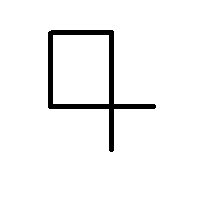
\includegraphics[width=5cm]{pic/1.png}
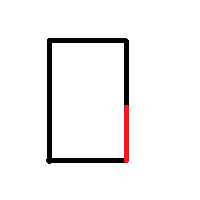
\includegraphics[width=5cm]{pic/2.png}

\includegraphics[width=5cm]{pic/3.png}

So we clarify the relations of the length of these lines in each circumstance, then the problem is solved.

The source code is shown in "Q3.cpp".

~\\
~\\

\end{enumerate}
%========================================================================
\end{document}
